%Version 3.1 December 2024
% See section 11 of the User Manual for version history
%
%%%%%%%%%%%%%%%%%%%%%%%%%%%%%%%%%%%%%%%%%%%%%%%%%%%%%%%%%%%%%%%%%%%%%%
%%                                                                 %%
%% Please do not use \input{...} to include other tex files.       %%
%% Submit your LaTeX manuscript as one .tex document.              %%
%%                                                                 %%
%% All additional figures and files should be attached             %%
%% separately and not embedded in the \TeX\ document itself.       %%
%%                                                                 %%
%%%%%%%%%%%%%%%%%%%%%%%%%%%%%%%%%%%%%%%%%%%%%%%%%%%%%%%%%%%%%%%%%%%%%

%%\documentclass[referee,sn-basic]{sn-jnl}% referee option is meant for double line spacing

%%=======================================================%%
%% to print line numbers in the margin use lineno option %%
%%=======================================================%%

%%\documentclass[lineno,pdflatex,sn-basic]{sn-jnl}% Basic Springer Nature Reference Style/Chemistry Reference Style

%%=========================================================================================%%
%% the documentclass is set to pdflatex as default. You can delete it if not appropriate.  %%
%%=========================================================================================%%

%%\documentclass[sn-basic]{sn-jnl}% Basic Springer Nature Reference Style/Chemistry Reference Style

%%Note: the following reference styles support Namedate and Numbered referencing. By default the style follows the most common style. To switch between the options you can add or remove “Numbered” in the optional parenthesis. 
%%The option is available for: sn-basic.bst, sn-chicago.bst%  
 
%%\documentclass[pdflatex,sn-nature]{sn-jnl}% Style for submissions to Nature Portfolio journals
%%\documentclass[pdflatex,sn-basic]{sn-jnl}% Basic Springer Nature Reference Style/Chemistry Reference Style
\documentclass[pdflatex,sn-mathphys-num]{sn-jnl}% Math and Physical Sciences Numbered Reference Style
%%\documentclass[pdflatex,sn-mathphys-ay]{sn-jnl}% Math and Physical Sciences Author Year Reference Style
%%\documentclass[pdflatex,sn-aps]{sn-jnl}% American Physical Society (APS) Reference Style
%%\documentclass[pdflatex,sn-vancouver-num]{sn-jnl}% Vancouver Numbered Reference Style
%%\documentclass[pdflatex,sn-vancouver-ay]{sn-jnl}% Vancouver Author Year Reference Style
%%\documentclass[pdflatex,sn-apa]{sn-jnl}% APA Reference Style
%%\documentclass[pdflatex,sn-chicago]{sn-jnl}% Chicago-based Humanities Reference Style

%%%% Standard Packages
%%<additional latex packages if required can be included here>

\usepackage{hyperref}
\usepackage{graphicx}
\usepackage{amsmath}
\usepackage{verbatim}
\usepackage{tcolorbox}
\usepackage[dvipsnames]{xcolor}
\usepackage{acro}
%%%%

%%%%%=============================================================================%%%%
%%%%  Remarks: This template is provided to aid authors with the preparation
%%%%  of original research articles intended for submission to journals published 
%%%%  by Springer Nature. The guidance has been prepared in partnership with 
%%%%  production teams to conform to Springer Nature technical requirements. 
%%%%  Editorial and presentation requirements differ among journal portfolios and 
%%%%  research disciplines. You may find sections in this template are irrelevant 
%%%%  to your work and are empowered to omit any such section if allowed by the 
%%%%  journal you intend to submit to. The submission guidelines and policies 
%%%%  of the journal take precedence. A detailed User Manual is available in the 
%%%%  template package for technical guidance.
%%%%%=============================================================================%%%%


\raggedbottom
%%\unnumbered% uncomment this for unnumbered level heads

\usepackage{acro}

\DeclareAcronym{ict}{
  short = ICT,
  long  = Information and Communication Technologies
}

\DeclareAcronym{vilt}{
  short = ViLT,
  long  = Virtual Intelligent Tutor
}

\DeclareAcronym{ai}{
  short = AI,
  long  = Artificial Intelligence
}

\DeclareAcronym{aied}{
  short = AIEd,
  long  = Artificial Intelligence in Education
}

\DeclareAcronym{ml}{
  short = ML,
  long  = Machine Learning
}

\DeclareAcronym{nlp}{
  short = NLP,
  long  = Natural Language Processing
}

\DeclareAcronym{llm}{
  short = LLM,
  long  = Large Language Model
}

\DeclareAcronym{rag}{
  short = RAG,
  long  = Retrieval-Augmented Generation
}

\DeclareAcronym{gpt}{
  short = GPT,
  long  = Generative Pre-trained Transformer
}

\DeclareAcronym{peft}{
  short = PEFT,
  long  = Parameter-Efficient Fine-Tuning
}

\DeclareAcronym{lora}{
  short = LoRA,
  long  = Low-Rank Adaptation
}

\DeclareAcronym{mas}{
  short = MAS,
  long  = Multi-Agent System
}

\DeclareAcronym{aose}{
  short = AOSE,
  long  = Agent-Oriented Software Engineering
}

\DeclareAcronym{abm}{
  short = ABM,
  long  = Agent-Based Modelling
}

\DeclareAcronym{bdi}{
  short = BDI,
  long  = Beliefs-Desires-Intentions
}

\DeclareAcronym{kpi}{
  short = KPI,
  long  = Key Performance Indicator
}

\begin{document}

\title[ViLT: A Retrieval-Augmented LLM Tutoring Framework for Subject-Specific Learning Support


\author*[1]{\fnm{Alberto} \sur{Fern\'andez-Isabel}}\email{alberto.fernandez.isabel@urjc.es}

\author[1]{\fnm{Isaac} \sur{Mart\'in de Diego}}\email{isaac.martin@urjc.es}

\author[1]{\fnm{Carmen} \sur{Lancho}}\email{carmen.lancho@urjc.es}

\author[2]{\fnm{Rub\'en} \sur{Fuentes-Fern\'andez}}\email{rfuentes@ucm.es}

\author[3]{\fnm{Ricardo J.} \sur{Ru\'iz-Gavir\'ia}}\email{ricardoruiz@unisinu.edu.co}

\affil*[1]{\orgdiv{Department of Computing and Statistics}, \orgname{Rey Juan Carlos University}, \orgaddress{\street{C/ Tulip\'an, s/n}, \city{M\'ostoles}, \postcode{28933}, \state{Madrid}, \country{Spain}}}

\affil[2]{\orgdiv{Research Group on Agent-based, Social \& Interdisciplinary Applications}, \orgname{Complutense University of Madrid}, \orgaddress{\street{ C/ Profesor Jos\'e Garc\'ia Santesmases 9}, \city{Madrid}, \postcode{28040}, \state{Madrid}, \country{Spain}}}

\affil[3]{\orgdiv{Department of Systems Engineering}, \orgname{Sinú-El\'ias Bechara Zain\'um University}, \orgaddress{\street{38th Street 1-37}, \city{Monter\'ia}, \postcode{230001}, \state{C\'ordoba}, \country{Colombia}}}

%%==================================%%
%% Sample for unstructured abstract %%
%%==================================%%

%\abstract{Nowadays, the job of teaching has adopted the \gls{ICT} for learning tasks in multiple areas of education. In this context, the most recent advances in \gls{AI} related to chatbots and \glspl{LLM} have been used only as assistants in a question \& answering solution from a global perspective. However, developing novel systems for detailed help with subjects and tutoring students to strengthen the knowledge acquired during class is a key issue. This paper presents \gls{ViLT}. It is a complete framework for tutoring students, collecting information on the syllabus of subjects, and producing a specific virtual expert based on \glspl{LLM}. This expert can explain related concepts, giving examples, procedures, and key details, thanks to the inclusion of a \gls{RAG} mechanism based on LangChain. Well-structured prompts guide these virtual tutors in acting as mentors and being coherent with the topics of the subjects. The functionalities of \gls{ViLT} are completed with a feedback module to evaluate the quality of the responses according to the request made. Educators can consult an integrated visualization dashboard to analyze the evolution of the course through different \glspl{KPI} extracted from the interactions with the virtual tutors. Several experiments have been conducted using subjects at Rey Juan Carlos University and Complutense University of Madrid in Spain, and Sin\'u-El\'ias Bechara Zain\'um University in Colombia. The results are promising, increasing the ability of students to reinforce concepts and easing the monitoring task of educators.}

\abstract{Teaching and learning processes increasingly rely on \ac{ict}, while recent advances in \ac{ai}, chatbots, and \acp{llm} have created new opportunities for personalized academic support. However, many \acp{llm}-based educational assistants remain general-purpose tools and are not explicitly grounded in the syllabus, materials, and pedagogical requirements of specific subjects. This paper presents \ac{vilt}, an integrated framework for deploying subject-specific virtual tutors based on \acp{llm} and \ac{rag}. \ac{vilt} enables educators to provide course materials that are processed and indexed to generate grounded answers aligned with each subject. The virtual tutor explains concepts, provides examples, and answers subject-related questions, while structured prompts constrain its behavior to the available educational context. The framework also incorporates a feedback module and a visualization dashboard that summarizes student interactions through \acp{kpi}, supporting educators in course monitoring and identification of difficult topics. Experiments conducted in subjects from three universities in Spain and Colombia show the feasibility of the framework and indicate positive perceptions from students and educators regarding its usefulness, precision, and pedagogical value.}


\keywords{Virtual Tutoring, Large Language Models, Human-Computer Interaction, Online Education, Concept Reinforcement}

%%\pacs[JEL Classification]{D8, H51}

%%\pacs[MSC Classification]{35A01, 65L10, 65L12, 65L20, 65L70}

\maketitle

\glsresetall

\section{Introduction}
\label{sec:intro}
Including and using technology in education is an open topic that evolves while trying to keep up with the rapid pace of the AI age \cite{ratheeswari2018information}. This evolution started with the inclusion of computers in the classrooms in elemental and higher schools at the beginning of the century. It was continued with specific computer science subjects, and later with tablets and mobile phones as support material in class.

On the other hand, groundbreaking educational methodologies have arisen during this period. Among them, e-learning \cite{liu2023towards} and gamification \cite{oliveira2023tailored} are some of the most successful thanks to their ability to produce periods of concentration in students and a certain level of fun while learning.

In the case of \gls{AI}, the most recent approaches based on \glspl{LLM} have provided support to the academic world (mainly universities and research centers). The impact has been similar for the educational community in high and elementary schools, including both educators and students \cite{kasneci2023chatgpt}. The adoption of these systems and their technology has been historically the fastest to be established in the world \cite{makridakis2023large}. This has occurred because \glspl{LLM} include chatbots with an inborn ability to interact at the human level. Moreover, they are excellent in duties like generating new text, rewriting paragraphs, and solving global questions (with a certain level of quality). In this sense, ChatGPT ((which uses different releases of \gls{GPT}) is the most widely known and used model \cite{lund2023chatting}.

However, these systems have some drawbacks. They have been trained with pieces of information from very different topics and domains. This makes them prone to make mistakes or produce imprecise answers. To alleviate this problem, fine-tuning processes are used to make these systems virtual experts in a specific domain. \gls{PEFT} techniques \cite{he2021towards}, and and more specifically \gls{LoRA} \cite{hu2021lora}, are used here. Nevertheless, fine-tuning techniques are not without problems, as they are very demanding in terms of computational resources, which makes it necessary to use specific machines or infrastructures to achieve an acceptable adaptation of the model. Moreover, \glspl{LLM} usually include some random factors (e.g. ``temperature'') that make them more or less prone to be creative in their answers (e.g. using different text forms), but also to make mistakes or invent information about a specific topic. These situations are called ``hallucinations'' and generate inconsistencies and problems in the provided solutions.

\gls{RAG} techniques \cite{gao2023retrieval} appear to address some of these issues. They take a user query and first retrieve information from trusted data sources, then provide both the user query and the relevant information to the \gls{LLM}, which uses this knowledge and its training data to create the answer. With this, \gls{RAG} creates more robust systems where the \gls{LLM} returns more precise and deterministic answers according to a topic and largely reduces the hallucination problems, without incurring in the high computational and financial costs associated with continuously training these models.

Taking advantage of these \gls{AI} technologies, this paper presents a novel framework called \gls{ViLT} to improve the quality of the learning process from both the perspective of educators and students. It provides virtual tutors who serve as always-available mentors to address subject-related doubts, similar to how a student would interact with an educator during a tutoring session. These virtual tutors of the system are based on \glspl{LLM} and are managed by intelligent agents that are part of a \gls{MAS} \cite{dorri2018multi}.

For each specific topic, the virtual tutor adapts using the content provided and reviewed by the educator through \gls{RAG} techniques. This ensures that the chatbot's responses align with the subject's content and requirements.

In addition, the system has a dashboard that tracks and summarizes all student interactions with the virtual tutor. This dashboard includes \glspl{KPI} related to: (1) usage data, such as how often each student uses the tool and the duration of their sessions, (2) information about the questions asked and the topics where students encounter more difficulties, and (3) the feedback of the students. Thanks to this dashboard, educators can monitor student interactions with \gls{ViLT} at any time and use the information to reinforce the most problematic concepts in the classroom or to schedule tutoring sessions with some students.

With these elements, the proposed framework provides provides a new dimension to the development of the course that benefits both students and educators. It improves the quality of the learning process with additional and tailored resources, keeps the educator in control, and can be adapted to the actual context.

Several experiments have been conducted with distinct degrees at Rey Juan Carlos University and Complutense University of Madrid in Spain, and Sin\'u-El\'ias Bechara Zain\'um University in Colombia. Similar subjects from Computer Science grades were analyzed, establishing similarities and detecting different strengths and weaknesses.

The rest of the paper is organized as follows. Section \ref{sec:background} embraces the foundations and technologies applied in this work. Then, Section \ref{sec:proposal} describes the framework. Section \ref{sec:experiments} presents some experiments that illustrate the system's application. Finally, Section \ref{sec:conclusions} discusses some conclusions and future lines of work.


\section{Background}
\label{sec:background}
The background of the proposed work lies in the tutoring task, the evolution of \gls{AI} and its inclusion in education in recent years, and how \glspl{LLM} have impacted society in general and the educational field in particular. Notice that these three concepts are the pillars of the proposal, building the \gls{ViLT} as a consequence of their joining.

Section \ref{sec:tutoring} addresses the relevant methodologies in education. It details how the tutoring task has evolved from standard techniques until reaching the most advanced systems. 
Section \ref{sec:ai} introduces typical approaches based on \gls{AI} in education, offering a chronological review that highlights how it has evolved into a key element today. Finally, Section \ref{sec:llm} tackles \glspl{LLM}, a disruptive and novel technology that has evolved to become one of the most useful tools.


\subsection{The evolution of tutoring}
\label{sec:tutoring}
Tutoring has traditionally been one of the most widely used strategies in the learning process. It helps students resolve questions or difficulties not fully understood during previous explanations. These tutoring sessions are typically short and personalized, facilitating a focused exchange of information between participants \cite{grey2020perceptions}. This technique has been extensively evaluated, highlighting its ability to increase students' competencies in most cases \cite{lopez2020school}. 

The tutoring process can be organized from two perspectives: the communication channel and the actors. In the first case, the tutoring task can take place directly in person through face-to-face meetings or using virtual communication channels. Face-to-face meetings are the most basic and typical procedure. Online tutoring, widely known as e-tutoring, emulates a face-to-face meeting \cite{kraft2022online}. This technique makes meeting scheduling easier, and although it has some drawbacks, it has shown similar results to face-to-face tutoring \cite{mare2021effectiveness}. In the second case, the actors are usually educators and students. However, this structure has evolved to peer tutoring, where students act as tutors or mentors of other students \cite{fernandez2023peer}. This approach relies on the assumption that students generally feel more at ease working with peers. Additionally, interacting with individuals of similar ages and experiences tends to be both easier and more effective \cite{thurston2020influence}. A relevant approach is reciprocal tutoring \cite{alemu2020improving}, which is an evolution of peer tutoring where actors play all roles, being able to solve problems and also raise questions.

In this context, the role of educators has increasingly been supplemented by computer systems acting as virtual mentors \cite{zhou1999practical}. These systems are capable of engaging in natural language conversations with students \cite{paladines2020systematic} and also understand complex queries \cite{rathore2020intelligent}. However, such approaches often lack specificity and can yield unpredictable outcomes. Therefore, it is key for educators to contribute their expertise to tailor these systems to the particular needs of each subject and, subsequently, verify their effectiveness.

These systems can use \gls{ML} models to produce adaptive learning, detect the weaknesses of the individuals who interact with them, and provide information about specific topics to reinforce their knowledge \cite{katz2021linking}. This is usually based on the automated classification of students according to determined features of interest such as assistance or doubts \cite{vsaric2023student}, which enables the development of student profiles and the identification of specific groups with similar weaknesses \cite{alshaikh2021ai}.

This paper introduces a system featuring intelligent tutors equipped with subject-specific knowledge, provided and validated  by the respective educators. The system integrates a \gls{MAS} alongside cutting-edge \gls{ML} techniques to support student learning. Thus, it maintains conversations in natural language, understanding specific questions, and providing detailed solutions. Integrating \glspl{LLM} has increased the quality of the dialogue and the versatility of the proposal.


\subsection{AI in the education}
\label{sec:ai}
\gls{AI} in education also called \gls{AIEd} is a branch inside the education area related to computer science. It is directly influenced by technological advances and the evolution of learning techniques \cite{chen2020artificial}. 

\gls{AIEd} consists of satisfying the needs of educators and experts in education providing intelligent systems. These systems are typically tools or applications specifically designed to assist with teaching tasks alongside educators during class or to offer support to students throughout the learning process. As such, they can be categorized into two perspectives based on their role in education: educator and student-oriented systems \cite{chen2022two}.

Educator-oriented systems have evolved in the last few years to facilitate the duties of educators. The most typical are related to revitalizing the classes, providing guidelines to educators, and elaborating documents (tests or exercises) according to a topic to learn. Well-known examples of these frameworks are tools such as Kahoot \cite{medina2017kahoot}, ClassDojo \cite{digiacomo2021students}, and Rexams library \cite{grun2009automatic}.

Student-oriented systems usually include specific trainers or problem solvers for the students. They can act as an information provider summarizing the relevant, emulate real environments, or develop games to promote the learning task of individuals through game-based techniques. Well-known examples of information providers are web search engines focused on education or academic tasks such as Google Scholar \cite{jacso2008google}, while intelligent systems are oriented to emulating real conditions (e.g., car driving and flight simulators) \cite{de2013analysis}. Furthermore, e-learning oriented to serious games and gamification are relevant game-based techniques \cite{tolks2024role}.

Alternatively, \gls{AIEd} can also be organized into three perspectives according to the role of the system \cite{ouyang2021artificial}: AI-directed, AI-supported, and AI-empowered. In the first case, intelligent systems represent and direct cognitive learning while learners are the recipients. In the second case, intelligent systems support learning while learners play as collaborators. In the third case, intelligent systems empower learning while learners are responsible for their improvement.

It is important to highlight the rise of \glspl{LLM}, and especially ChatGPT \cite{kasneci2023chatgpt} nowadays. These systems have revolutionized education, allowing students to produce documents, works, and very different novel content without human intervention. Moreover, from the educator´s perspective, they are useful in developing new subject content, such as summaries and practice exercises for assessments \cite{orenstrakh2023detecting}.

This paper presents a framework that includes specialized virtual tutors for each subject. It is focused on the perspective of the learners being mainly an AI-empowered system. These tutors are intelligent agents that include \glspl{LLM} adapted to provide specific information.


\subsection{Large Language Models}
\label{sec:llm}
\glspl{LLM} have appeared to revolutionize the \gls{AI} era, radically changing the landscape and the \gls{NLP} techniques \cite{hadi2023large}. They use a large amount of unlabeled textual data to be trained to understand the syntax and semantics of the language.

These systems incorporate a deep learning algorithm to address different \gls{NLP} tasks such as text translation, word prediction, text generation, and conversational agents \cite{zhao2023survey}. Among these tasks, textual annotations (labeling the type of a word according to the sentence) \cite{he2023annollm} and text generation (from an initial sentence or a specific topic) are those where the improvement has been highly significant \cite{min2023recent}.

The deep learning algorithm consists of a specific type of neural network called transformers that use attention methods \cite{niu2021review}. Transformers are built through a set of elements: input embeddings, positional encoding modules, encoders, output embeddings, decoders, linear layers, and softmax layers \cite{vaswani2017attention}.

Well-known examples of these systems are \gls{GPT} \cite{floridi2020gpt} (from OpenAI) and PaLM \cite{anil2023palm} (from Google). Both are closed-source models that cannot easily adapt to a new context. However, new \glspl{LLM} have recently been developed as open source systems. Well-known instances of them are: Llama \cite{lu2023llama}, Gemma 2 \cite{team2024gemma}, Qwen 2.5 \cite{hui2024qwen2}, and Mistral 2 \cite{jiang2023mistral}.

Unlike previously developed language models, \glspl{LLM} can achieve high prediction quality in few-shot and zero-shot scenarios without aggregating new extensive training data or model fine-tuning \cite{kojima2022large}. However, in some cases, the knowledge they can provide is too general \cite{liu2023summary}. In such a scenario, fine-tuning operations can produce accurate results in specialized domains, but at the cost of high computational costs. This is the case in fields like health care, where terminology and definitions are specific \cite{singhal2023large}, or in code generation across multiple programming languages, where general templates or detailed functions are well established \cite{wang2023codet5}.

Alternatively, some methods have emerged to reduce the effort of adapting \glspl{LLM} to specific domains and tasks. \gls{PEFT} techniques \cite{he2021towards} can fine-tune \glspl{LLM} by updating only a small set of parameters. On the other hand, \gls{RAG} \cite{gao2023retrieval} techniques can adapt \glspl{LLM} to avoid the update process by providing new knowledge to the model by inserting embeddings directly into the prompt.

\gls{ViLT} is a system that works with open source \glspl{LLM} and with \gls{GPT} releases. \glspl{LLM} can be automatically adapted to the specific domain of the subject. This adaptation has been achieved using \gls{RAG} techniques to include new knowledge to cover the syllabi of subjects, avoiding excessive consumption of resources produced by a fine-tuning process. This design provides high flexibility, easing the tutor's adaptation to the needs of the course.


\section{Proposed Framework}
\label{sec:proposal}
The proposed framework called \gls{ViLT} focuses on virtual tutoring and monitoring of student tasks, effectively addressing the needs of both students and educators throughout the course. These tutoring activities are managed by virtual tutors. Each tutor is equipped with a specialized \gls{LLM} customized to the syllabus requirements of the specific subject (see Fig. \ref{fig:chatbot}).

\begin{figure}[t!]
	\centering
	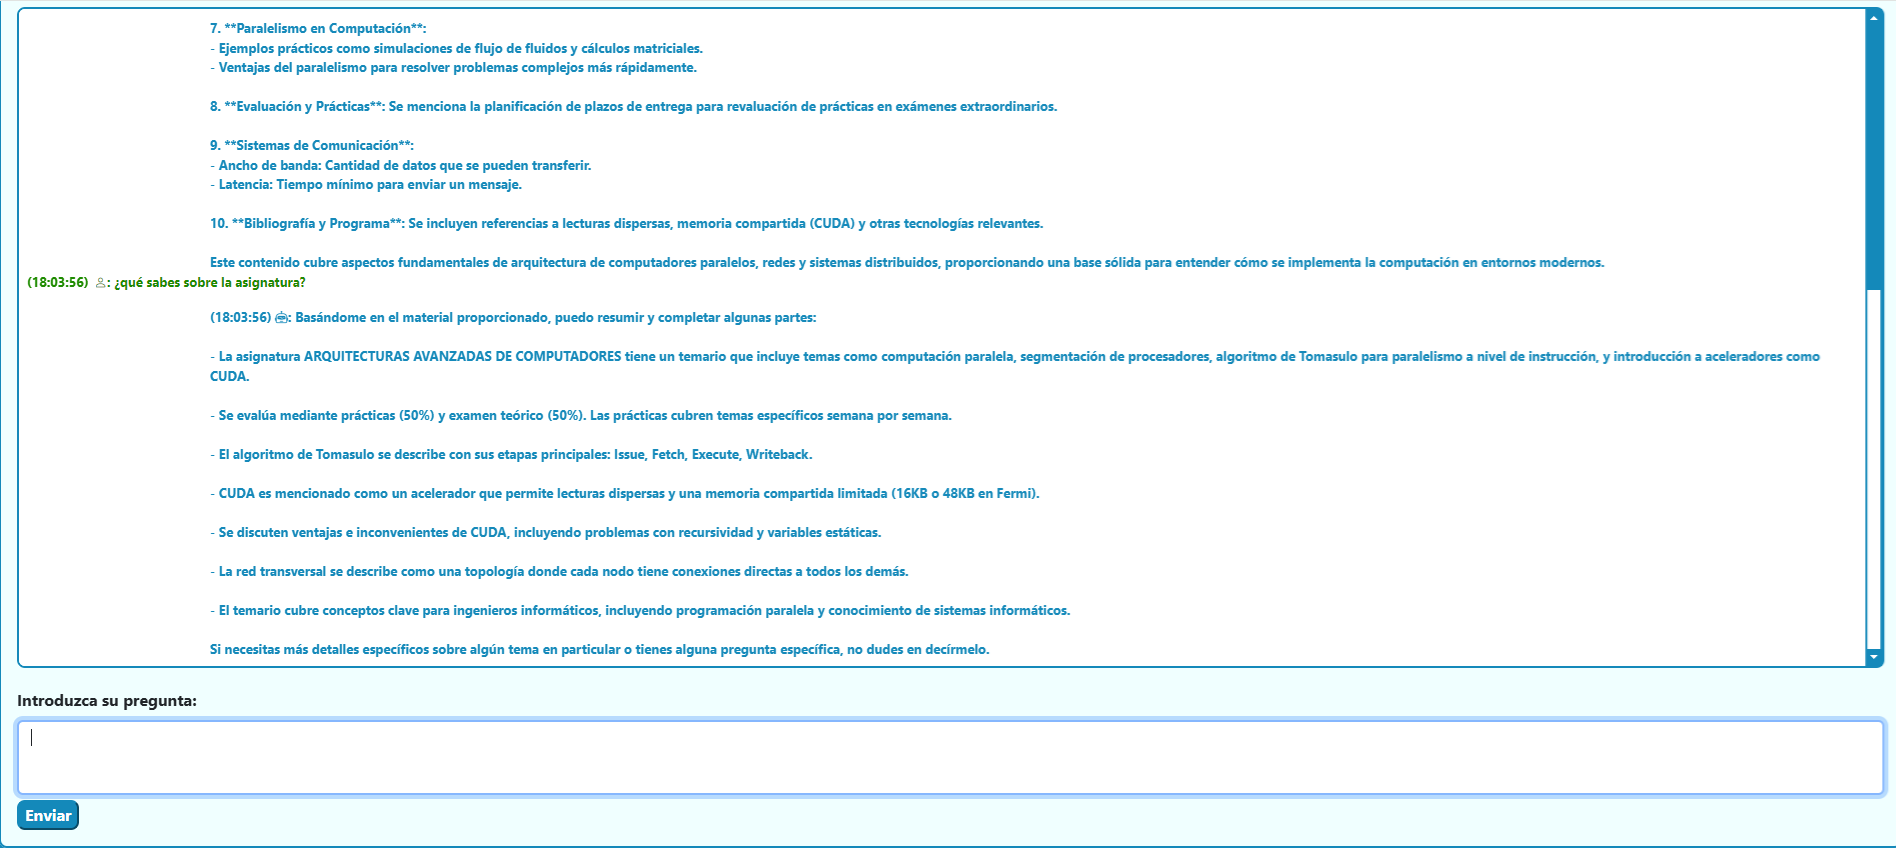
\includegraphics[scale=0.24]{figs/chatbot.png}
	\caption{Excerpt of the \gls{ViLT} chatbot in Spanish language.}
	\label{fig:chatbot}
\end{figure}

A \gls{MAS} controls and distributes the main tasks of \gls{ViLT}. These agents play the roles of general manager, chatbot manager, and embedding manager. 

The system has two main workflows: the main workflow corresponds to the interaction with the different users in real-time, and the updating information workflow to the tasks in batch to produce new embedded releases based on the syllabus of the subjects.

The roles of users included in \gls{ViLT} are: administrator (in charge of adding information about subjects and degrees), educator (who submits material related to the syllabus of subjects and visualize individual and collective statistics about the development of the course), and students (that interact with the chatbot in a request-answer cycle and provide feedback about the quality of the proposal).

\subsection{Architecture}
\label{sec:architecture}
The \gls{ViLT} architecture is based on completely distributed and isolated platforms for each target subject. These platforms are dynamic (i.e., the system creates or destroys them as needed) and have six modules and three individual databases (see Fig. \ref{fig:vilt}). They connect via an API to the \gls{LLM} server that hosts the corresponding \gls{LLM} (represented in the figure with a database icon too).

\begin{figure}[t!]
	\centering
	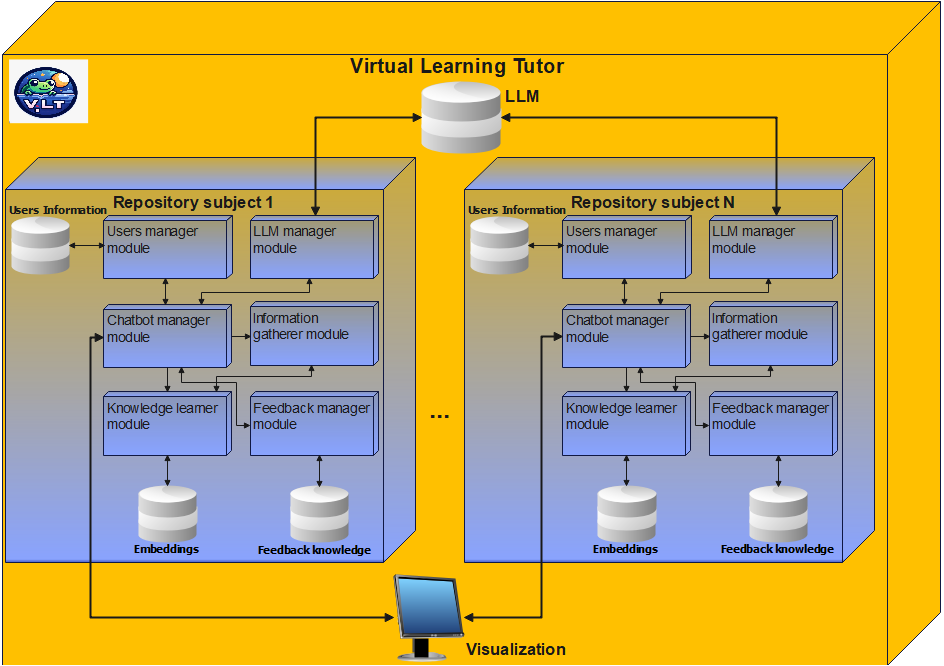
\includegraphics[scale=0.5]{figs/vilt.png}
	\caption{Overview of the \gls{ViLT} architecture.}
	\label{fig:vilt}
\end{figure}

The modules are: the \emph{LLM manager}, the \emph{Chatbot manager}, the \emph{Information gatherer}, the \emph{Knowledge learner}, the \emph{User´s manager}, and the \emph{Feedback manager}. The core of the system comprises the first four modules. They are managed by a \gls{MAS}, where intelligent autonomous agents based on the \gls{AOSE} architecture \cite{abdalla2021agent} organize and distribute actions and decisions.

On the other hand, the databases are: \emph{Embeddings} (i.e., a chroma database with the vectors of the syllabus for the subject \cite{kukreja2024performance}), \emph{Feedback knowledge} (i.e., knowledge obtained from the opinion of students who use the system in the subject) and \emph{Users information} (i.e., profile details of students and educators who are part of the subject). Notice that a visualization module completes the system in the front-end layer.

\begin{figure}[t!]
	\centering
	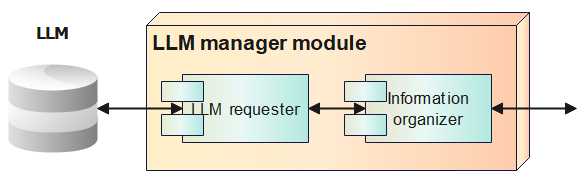
\includegraphics[scale=0.5]{figs/llm.png}
	\caption{The \emph{LLM manager} module and its components.}
	\label{fig:llm}
\end{figure}

Regarding the components of the modules, the \emph{LLM manager} module loads the corresponding \gls{LLM} and integrates the \gls{RAG} embeddings into it. Then, it manages the requests and answers between users and the chatbot. This module comprises two components: the \emph{LLM requester} component and the \emph{Information organizer} component. The first component addresses the actual communication with the user, while the second component establishes the structure of the environment (configuration of the parameters of the \gls{LLM} and the \gls{RAG} embeddings integration).

\begin{figure}[t!]
	\centering
	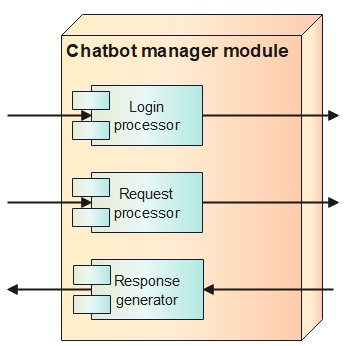
\includegraphics[scale=0.5]{figs/cmm.png}
	\caption{The \emph{Chatbot manager} module and its components.}
	\label{fig:cmm}
\end{figure}

The \emph{Chatbot manager} module presents the most relevant features of the system, acting as a bridge between the visual interface and the \gls{LLM}. It comprises three components: \emph{Login processor}, the \emph{Request processor}, and the \emph{Response generator}. The first only captures the login information to provide it to the \emph{User manager} module. The other ones generate the internal structure to establish communication between the chatbot and the users, produce the corresponding prompt, render the text to the specific format according to the used language, and correct possible typos.

\begin{figure}[t!]
	\centering
	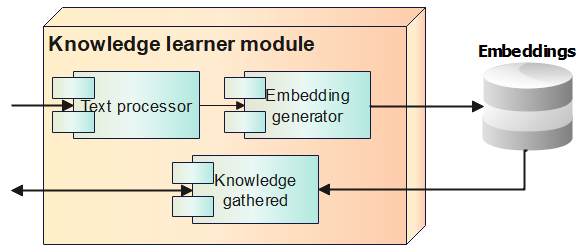
\includegraphics[scale=0.5]{figs/klm.png}
	\caption{The \emph{Knowledge learner} module and its components.}
	\label{fig:klm}
\end{figure}

The \emph{Knowledge learner} module is related to the learning flow of the system (i.e., the generation of the embeddings used for the RAG process), and the main work of the chatbot (i.e., the integration of the RAG using the embeddings and the \gls{LLM}). It comprises three components: the \emph{Text processor} component, the \emph{Embedding generator} component, and the \emph{Knowledge gatherer} component. The first component gathers information from the syllabus provided by educators extracting the textual content. The syllabus can have different file formats (e.g., Excel, Word, or PDF). The second component produces embeddings in a specific format (fast embeddings stored in a chroma database), having a maximum length value of $512$, and a similarity threshold value of $0.1$ with $k=20$. The third component collects and organizes the embeddings used by the \emph{LLM manager} module.

\begin{figure}[t!]
	\centering
	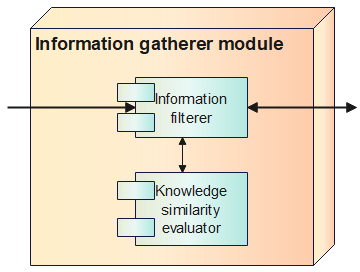
\includegraphics[scale=0.5]{figs/igm.png}
	\caption{The \emph{Information gatherer} module and its components.}
	\label{fig:igm}
\end{figure}

The \emph{Information gatherer} module works with the \emph{Knowledge gatherer} module in particular. It analyzes the information collected from the different syllabi detecting possible repeated material in the subjects or errors in the files provided by educators. It comprises two components: the \emph{Information filterer} component and the \emph{Knowledge similarity estimator} component. Both components collaboratively assume the task. The first component is the leader of the process, while the second component is the specialist in detecting repetitions.

\begin{figure}[t!]
	\centering
	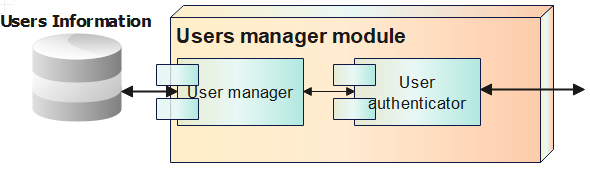
\includegraphics[scale=0.5]{figs/umm.png}
	\caption{The \emph{Users manager} module and its components.}
	\label{fig:umm}
\end{figure}

The \emph{Users manager} module supervises the information about the profiles of the registered users of the system. This module comprises two components: the \emph{User manager} component and the \emph{User authenticator} component. The first component addresses storage and retrieval tasks related to user information. These users are filtered according to the subject, the career, and the role (student, educator, or administrator). The second component obtains information about the credentials and confirms that users are registered in the database.

\begin{figure}[t!]
	\centering
	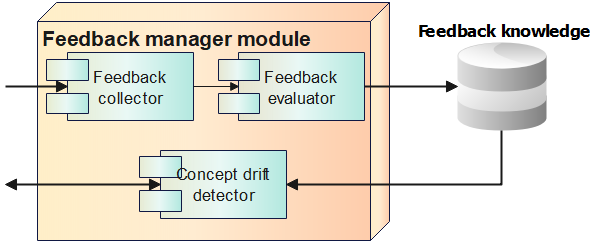
\includegraphics[scale=0.5]{figs/fmm.png}
	\caption{The \emph{Feedback manager} module and its components.}
	\label{fig:fmm}
\end{figure}

The \emph{Feedback manager} module gathers the students' opinions about the system. It includes three different components: the \emph{Feedback collector} component, the \emph{Feedback evaluator} component, and the \emph{Concept drift detector} component. The first component obtains the information directly from the visual interface, while the second organizes the feedback stored in the database. The third component detects possible problems with the learned concepts or weaknesses in specific parts of the syllabus during the development of the subject.

\begin{figure}[t!]
	\centering
	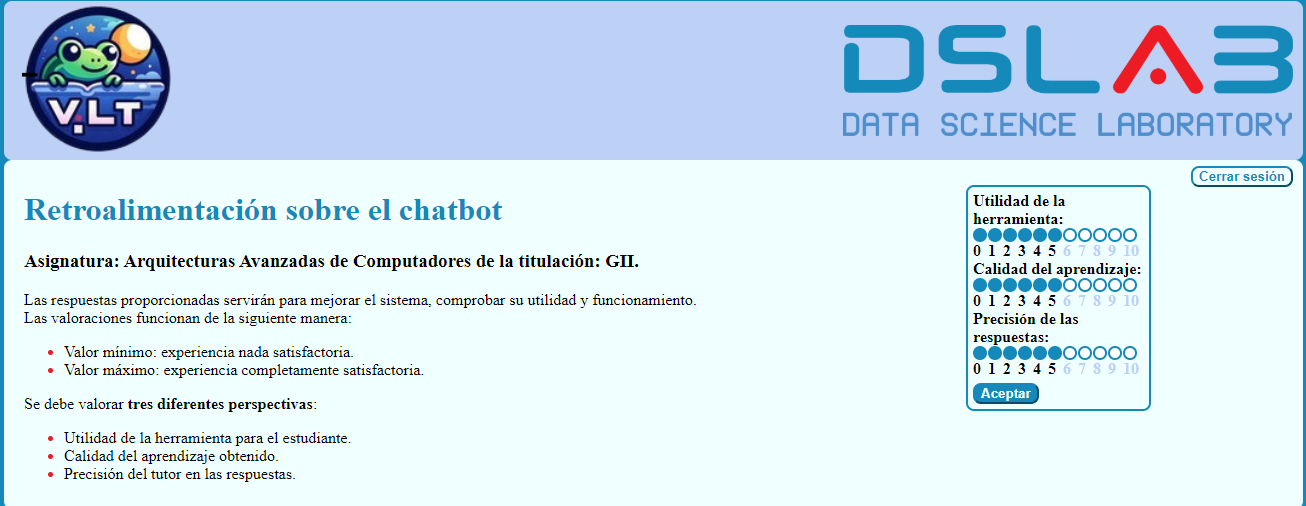
\includegraphics[scale=0.34]{figs/feedback.png}
	\caption{Feedback screen to evaluate the performance of the chatbot.}
	\label{fig:feedback}
\end{figure}

\begin{figure}[t!]
	\centering
	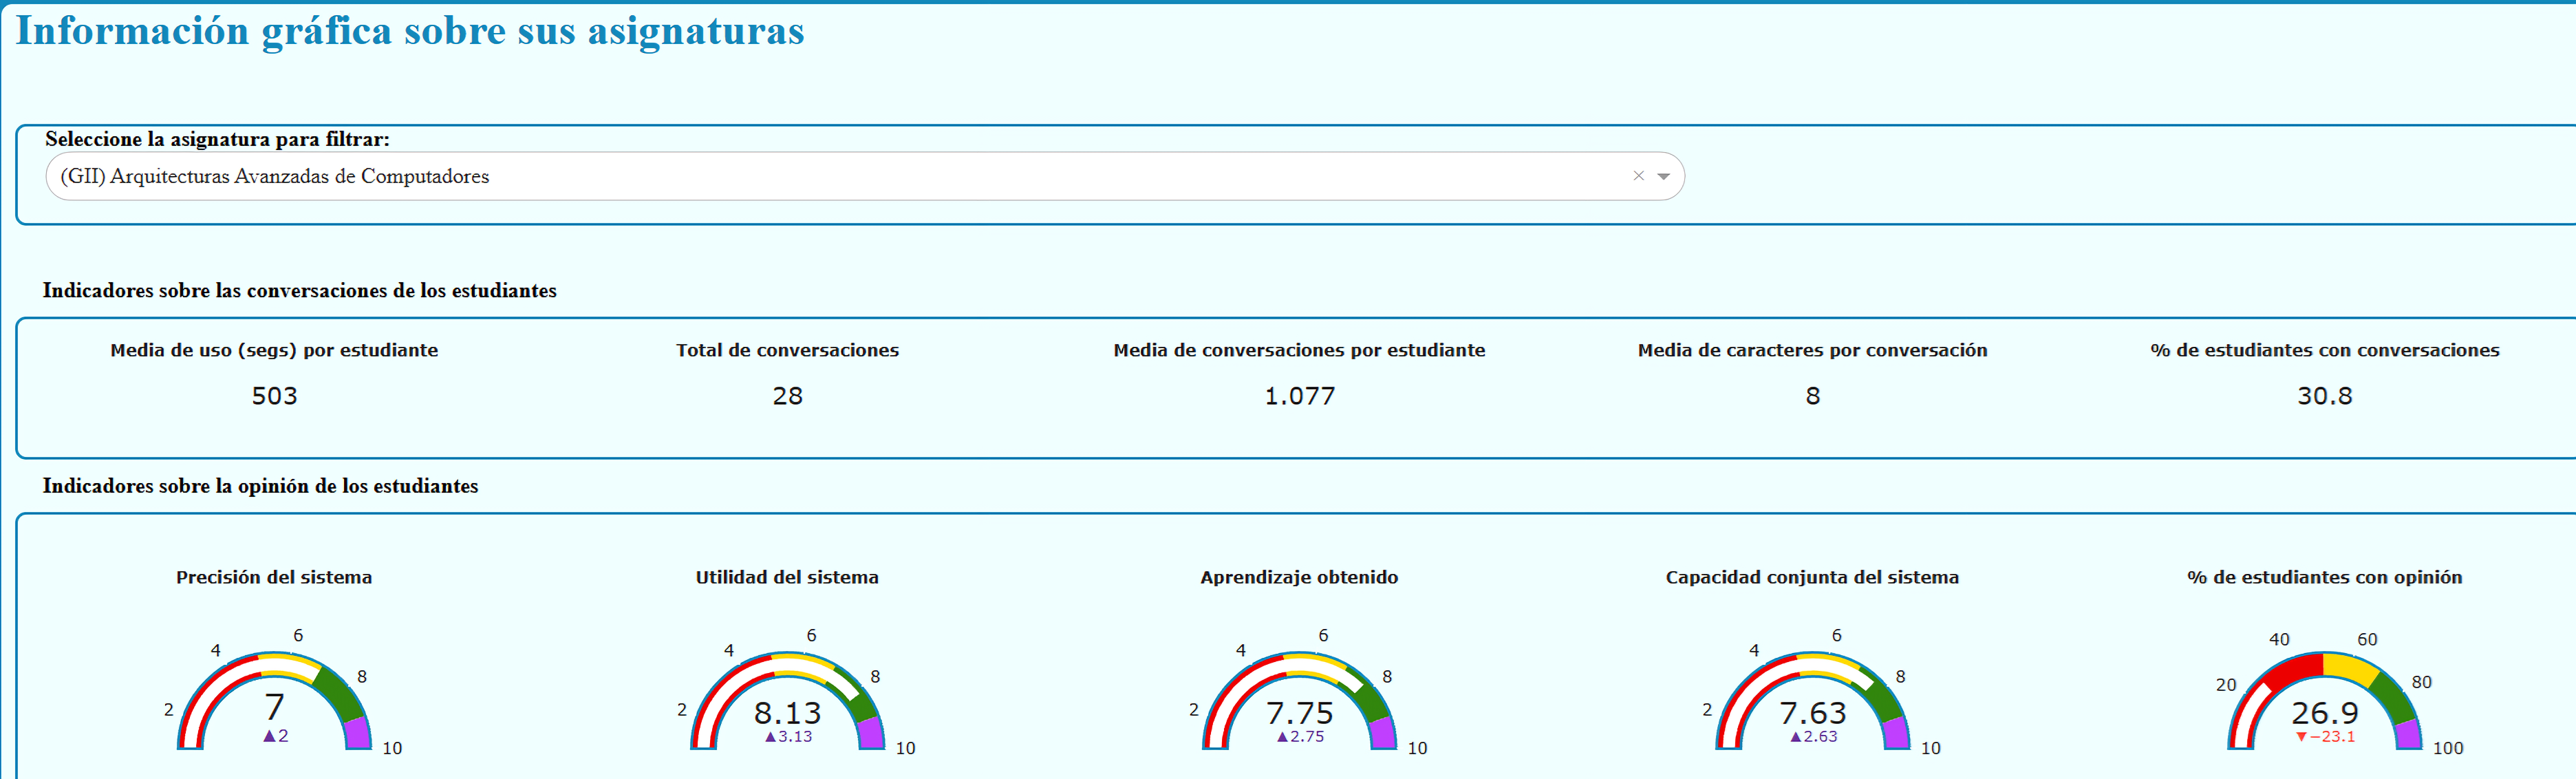
\includegraphics[scale=0.09]{figs/evaluation1.png}
	\caption{Global \glspl{KPI} provided by the \gls{ViLT} dashboard.}
	\label{fig:eval1}
\end{figure}

\begin{figure}[t!]
	\centering
	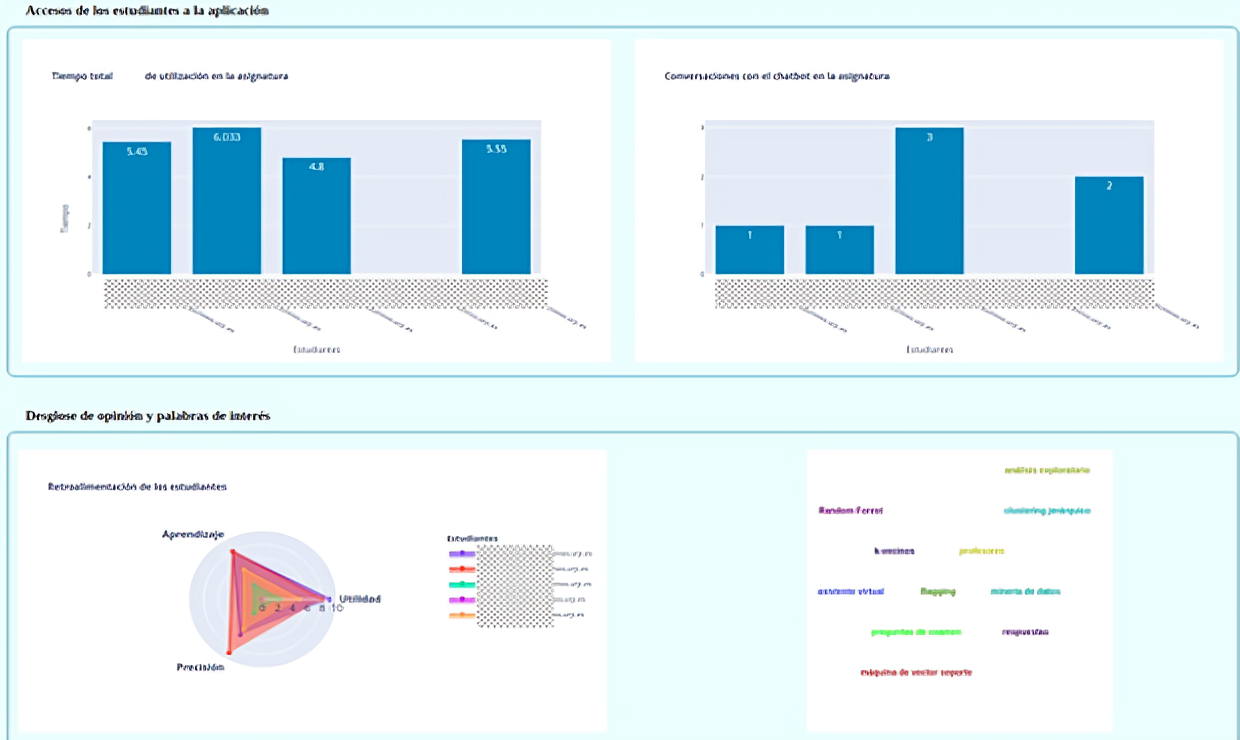
\includegraphics[scale=0.27]{figs/evaluation2.png}
	\caption{Filterable \glspl{KPI} provided by the \gls{ViLT} dashboard (anonymous email addresses).}
	\label{fig:eval2}
\end{figure}

The information collected regarding the feedback obtained by the tool consists of three perspectives that evaluate the system: the precision and the utility of responses, and the ability to make students learn (see Fig. \ref{fig:feedback}). In addition, the system collects \glspl{KPI} from students, such as the number of dialogues, average time per conversation with the chatbot (individually and collectively), and the most relevant keywords. This information is shown to educators through a dashboard, allowing educators to understand the evolution of students and to highlight specific needs. These \glspl{KPI} are grouped into two categories: global \glspl{KPI} (i.e., all the students of the subject) and filterable \glspl{KPI} (some students or individually). Figure \ref{fig:eval1} and Figure \ref{fig:eval2} illustrate excerpts of the dashboard and the different \glspl{KPI}.

\subsection{Multi-agent system}
\label{sec:mas}

\begin{figure}[t!]
	\centering
	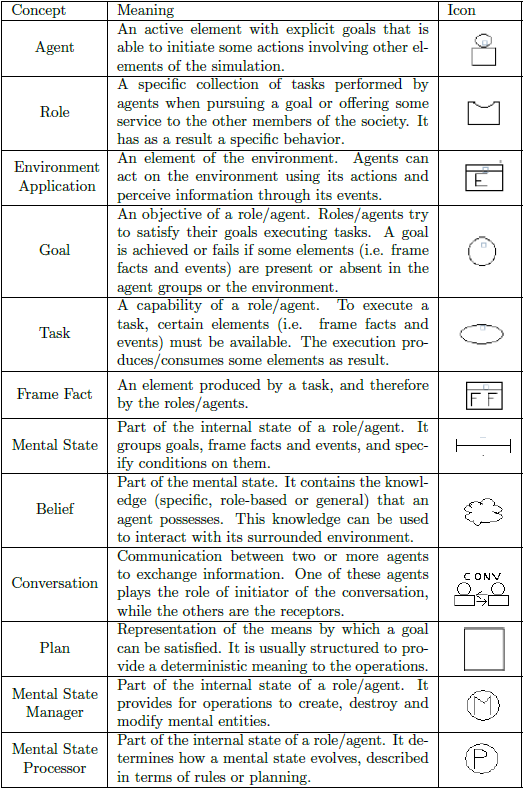
\includegraphics[scale=0.6]{figs/agentstable.png}
	\caption{Main concepts of INGENIAS for developing the \gls{MAS}.}
	\label{fig:agents}
\end{figure}

This section details the \gls{MAS} that implements the most relevant tasks of the \gls{ViLT} framework (the four main modules). The design of the \gls{MAS} follows INGENIAS \cite{gomez2010model}, a well-known \gls{ABM} methodology \cite{salmon2022agent} that includes \gls{AOSE}. In this sense, the proposal considers the \gls{BDI} model \cite{archibald2024quantitative}, where each agent has a mental state, believes, and plans to satisfy the main goal through specific tasks (see Fig. \ref{fig:agents}). The \gls{MAS} implementation has been addressed using SPADE \cite{palanca2022flexible}.

\begin{figure}[t!]
	\centering
	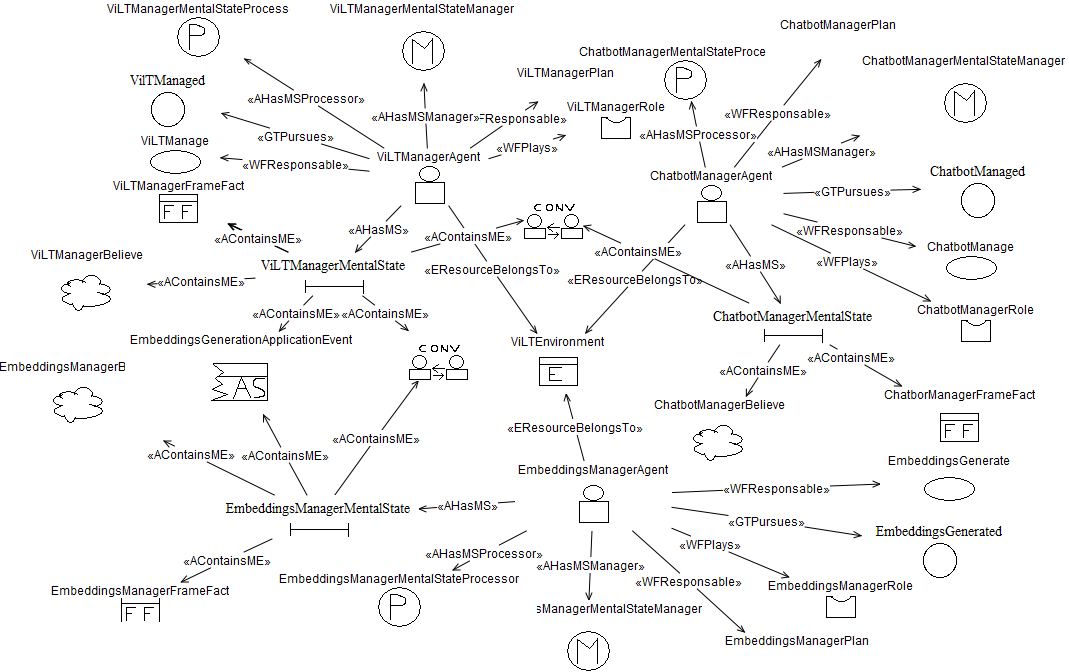
\includegraphics[scale=0.42]{figs/viltagents.png}
	\caption{Model of entities involved in the \gls{MAS}.}
	\label{fig:viltagents}
\end{figure}

Agents play three roles in managing the interactions between chatbots, users and the textual content gathered from the syllabus for each subject. The global manager for a subject is \emph{ViLT Manager Agent}, the chatbot responsible is \emph{Chatbot Manager Agent}, and the agent responsible for producing the embeddings for the \gls{RAG} system is \emph{ Embeddings Manager Agent} (see Fig. \ref{fig:viltagents}).

Regarding the goals, the \emph{ViLT Manager Agent} has \emph{ViLT managed} as the main goal, while the \emph{Chatbot Manager Agent} must satisfy the \emph{Chatbot managed} main goal. In the case of \emph{Embedding manager agent}, the main goal is \emph{Embeddings generated}. These goals include the actions for all the subjects addressed by the \gls{ViLT} framework.

\begin{figure}[t!]
	\centering
	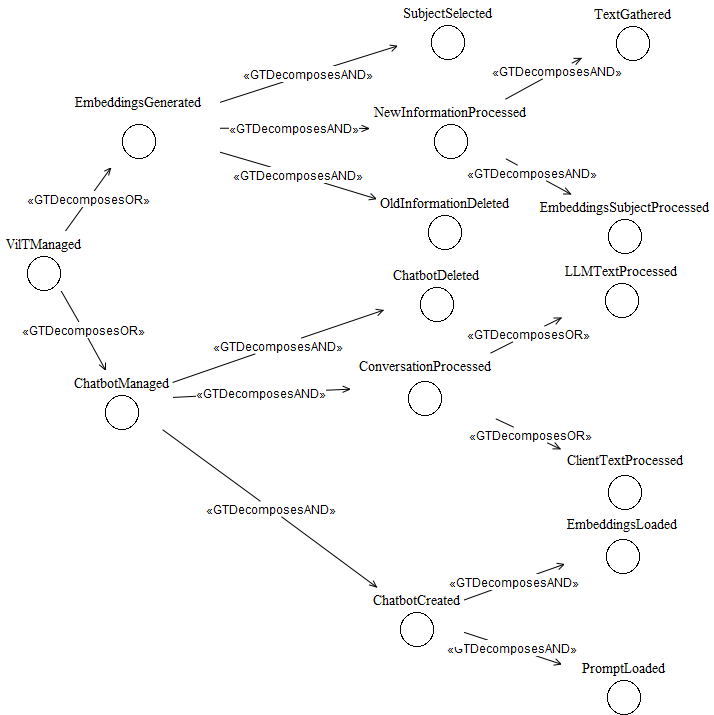
\includegraphics[scale=0.45]{figs/viltgoals.png}
	\caption{Hierarchical structure of goals in the \gls{MAS}.}
	\label{fig:goals}
\end{figure}

These goals are decomposed into others with simpler and more specific actions to achieve (see Fig. \ref{fig:goals}). The satisfaction of these child goals produces the satisfaction of the goal immediately higher in the hierarchical level. Thus, the \emph{ViLT managed} goal is decomposed into the \emph{Chatbot managed} and \emph{Embeddings generated} goals. In this case, it is only relevant that one of these goals is satisfied to satisfy the higher goal (i.e., the main goal of \gls{MAS}). These intermediate goals are also decomposed. The \emph{Chatbot managed} is composed of three goals that all need to be satisfied: \emph{Chatbot deleted}, \emph{Conversation processed}, and \emph{Chatbot created}. These goals control the lifecycle of a chatbot for each subject. Moreover, the \emph{Conversation processed} goal is decomposed into the goals that manage the conversation: \emph{LLM text processed} and \emph{Client text processed}. In the same way, the \emph{Chatbot created} is decomposed into \emph{Embeddings loaded} and \emph{Prompt loaded} goals, which control the correct loading of the necessary features to start the conversation with the chatbots of \gls{ViLT}. On the other hand, the \emph{Embeddings generated} goal is decomposed into three goals that must be satisfied: \emph{Subject selected}, \emph{New information processed}, and \emph{Old information deleted}. These goals tackle the generation of the embeddings, processing new information to include, and deleting ancient releases of embeddings.


\subsection{Workflow}
\label{sec:workflow}
The \gls{ViLT} framework has two main workflows: the main user workflow and the embeddings generation workflow. The first is interactive and includes all the tasks the system achieves (see Fig. \ref {fig:workflow}). The second supports these tasks, covering the generation or updating process of the embeddings for each subject, and it occurs automatically in batch.

The user workflow starts with a login, where the role of the users (admin, educator, or student) is filtered. If the user is a student, the tool allows only using the chatbot (requests and answers). Then, when the students do not have more requests, the feedback about the session is retrieved, and they can log out. 

If the user is an educator, the framework provides features to include new material in the syllabus of subjects (those in which the educator participates) or delete it if necessary. The dashboard can be loaded to visualize the evolution of subjects. Once educators have enough information or modifications have been made to the syllabus of their subjects, they can log out.

Finally, the system provides different management operations if the user has the admin role. Among them, the most relevant are the creation, modification, or deletion of a syllabus for a subject, the modification of the students and educators of a subject, and the creation, modification, or deletion of users in the system.

\begin{figure}[t!]
	\centering
	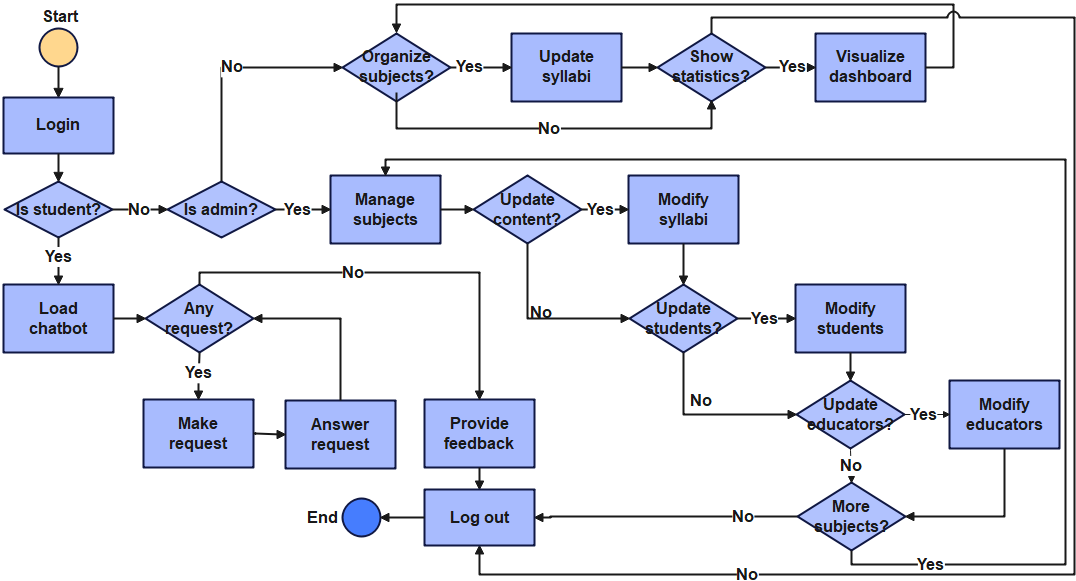
\includegraphics[scale=0.42]{figs/workflow.png}
	\caption{The user main workflow of the \gls{ViLT} framework.}
	\label{fig:workflow}
\end{figure}


\section{Experiments}
\label{sec:experiments}
The \gls{ViLT} framework has been developed to be launched on virtual platforms of universities. Before reaching this stage, several experiments were carried out to demonstrate the system's feasibility. The selected institutions were Rey Juan Carlos University and Complutense University of Madrid in Spain, along with Sin\'u-El\'ias Bechara Zain\'um University in Colombia. This selection was based on their existing collaboration agreements and the use of equivalent languages. Moreover, their computer science programs include similar subjects, facilitating comparative analysis. The ethics committee of Rey Juan Carlos University approved the \gls{ViLT} project and the corresponding experiments. 

These experiments are organized into four case studies conducted between June $2024$ and December $2024$. The first tackles the loading stage of the corresponding educators, students, and syllabi for the subjects. The second uses the syllabus of the subjects and loads different \glspl{LLM} to evaluate the best option between these models to interact with students. Thus, educators worked with the \glspl{LLM} using a set of requests to analyze the chatbots' responses. The third experiment addresses the quality and usability of the chatbot using the feedback provided by students. Finally, the fourth presents the dashboard features to achieve a global analysis of the subjects to detect weaknesses (individually or collectively) and similar patterns between subjects.

\subsection{System set-up and information loading stage}
\label{sec:setup}
In this first experiment, some subjects have been selected to be included in the \gls{ViLT} framework. Then, educators and students were registered as users with the corresponding roles. Later, the educators loaded the documents, which are part of the syllabus and study guide of the subjects. These documents included all course material, covering topics, the evaluation process, and the educator profile in PDF and Word formats. After that, the system automatically produced the embeddings for each syllabus using the LangChain features \cite{auffarth2023generative}.

Regarding the subjects, those selected from the Rey Juan Carlos University were \emph{Statistical Inference} in the Degree of Data Science and Engineering ($34$ students), \emph{Advanced Architectures of Computing} in the Degree of Computer Science ($15$ students), and \emph{Data Mining} in the Degree of Mathematics ($4$ students). Furthermore, the subject selected from the Complutense University of Madrid was \emph{Artificial Intelligence} in the Double Degree of Mathematics and Computer Science ($31$ students). Lastly, the subjects selected from the Sin\'u-El\'ias Bechara Zain\'um University were \emph{Probability and Statistics} ($23$ students), and \emph{Applied Computation} ($18$ students) in the Degree of System Engineering. In this way, $125$ students participated in the experiments. Notice the heterogeneity in the number of students, having subjects with several students and others with few from different levels.

Finally, the admins confirmed the correct configuration of the system, being ready to interact with educators and students in real cases. \gls{ViLT} used the API of \gls{GPT} 3.5 turbo as \gls{LLM} for the chatbot configuration by default. This decision is detailed in the next experiment.

\subsection{Selection of the chatbot model}
\label{sec:selection}
For this experiment, five different \glspl{LLM} have been tested by $6$ educators from the subjects previously indicated. These models are: \gls{GPT} $4$, \gls{GPT} $3.5$ turbo, Llama $3.1$, Gemma $2$, and Qwen $2.5$. The \gls{GPT} models used the OpenAI API \cite{kublik2023gpt}, while open source models were orchestrated through an Ollama server \cite{astekin2024comparative}. Parameters such as temperature have been configured to avoid hallucinations as much as possible.

Regarding the prompts, two equivalent prompts were built following the preferences of each type of participant model and how they understand the input orders. Thus, one of the prompts was designed to be better understood by the \gls{GPT} models, while the other was configured to focus on the Ollama open source models. Next, both prompts are shown.

\begin{tcolorbox}[colback=White, title=Prompt oriented to GPT models]
	\begin{verbatim}
		Accomplish accurately the next instructions:
		1) You are a teacher explaining to a student.
		2) Never use LaTeX symbols or backslashes.
		3) Spanish is the main language, but be ready for others.
		4) You must be respectful and honest, dedicated to 
		providing an accurate and informative response based
		solely and strictly on the provided context 
		((delimited by <ctx></ctx>)).
		5) The context represents a subject. Do not answer 
		questions outside of the subject.
		6) You can support your answers with code in various
		programming languages.
		<ctx>
		CONTEXT:
		{context}
		</ctx>
		
		QUESTION:
		{input}
		
		ANSWER:
	\end{verbatim}
\end{tcolorbox}

\begin{tcolorbox}[colback=white, title=Prompt oriented to Ollama open source models]
	\begin{verbatim}
		[INST]
		Accomplish accurately the next instructions:
		1) You play the role of a teacher called ViLT.
		Be polite and act like humans.
		2) Never use LaTeX symbols or backslashes.
		3) The answer must be precise, clear, detailed 
		and only contain one answer. Do not invent,
		4) The context is the content of the subject.
		5) You could provide examples in programming code 
		only if you are asked for them.
		6) Spanish is the native language, but be ready for others.
		[/INST]
		[INST] {input}
		Context: {context}
		Answer:
		[/INST]
	\end{verbatim}
\end{tcolorbox}

The performance of the models is estimated according to the scores provided by the educators in $4$ different dimensions: timeline (i.e., questions about the temporal organization of the subject, e.g., \emph{what is the main topic in the tenth week of the subject?}), evaluation (i.e., how the subject is evaluated following the study guide instructions, e.g., \emph{what are the most relevant aspects of the subject?}), content (i.e., concepts, theory, and examples related to the subject, e.g., \emph{could you accompany the explanation with source code?}), and trap (i.e., questions beyond the scope of the subject, e.g., \emph{what is an elephant?}).

Each dimension is evaluated in a range [$1$, $5$] (providing only integer numbers) where $1$ indicates a bad opinion and $5$ indicates an excellent opinion in the dimension. These values are obtained following a set of guided requests made to \glspl{LLM}, considering key questions about the concepts of the subject and the study guide, and specific examples reflected in the source code or equations included in the syllabi (see Table \ref{tab:evaluations}).

The results clearly illustrated that open source \glspl{LLM} performed worse when they had to provide the correct answers. Among them, Qwen $2.5$ stands out for the amount of information it provides beyond the scope of the subject. Gemma $2$ gets a better performance but the behavior is similar, presenting some hallucinations in the answers. Llama $3.1$ improves the results but its performance is far from both \gls{GPT} models.

In the case of \gls{GPT} models, their performance is similar, with \gls{GPT} $4$ being slightly better than \gls{GPT} $3.5$ turbo. This result is acceptable due to the nature of the models, being \gls{GPT} $4$ a more modern and larger version. However, the decision was to use \gls{GPT} $3.5$ turbo because the performance difference between both releases is low and the economical cost of deployment on a virtual platform for students is lower.

\begin{table}[t!]
	\centering
	\begin{tabular}{|l|l|l|l|l|l|}
		\hline
		\textbf{Model}     & \textbf{Timeline} & \textbf{Evaluation} & \textbf{Content} & \textbf{Trap} & \textbf{Performance}\\ \hline
		\textbf{GPT 4}     & \textbf{5.0} & \textbf{4.6} & \textbf{4.8} & \textbf{5.0} & \textbf{0.97} \\ \hline
		\textbf{GPT 3.5}   & $5.0$ & $4.4$ & $4.4$ & $5.0$ & $0.94$ \\ \hline
		\textbf{Llama 3.1} & $2.2$ & $2.0$ & $1.0$ & $3.0$ & $0.41$ \\ \hline
		\textbf{Gemma 2}   & $1.8$ & $1.2$ & $1.0$ & $1.8$ & $0.29$ \\ \hline
		\textbf{Qwen 2.5}  & $1.2$ & $1.4$ & $1.0$ & $1.2$ & $0.24$ \\ \hline
	\end{tabular}
	\caption{Average evaluations made by the educators in their subjects using the proposed models.}
	\label{tab:evaluations}
\end{table}

\subsection{Feedback analysis from students}
\label{sec:feedback}
This experiment evaluates the quality of the system from the student's perspective. The evaluation is based on the feedback provided by students after completing a tutoring session with the chatbot for a specific subject. Thus, in this scenario, \gls{ViLT} is examined through the lens of the student experience.

The feedback value (integers in a range [0, 10]) was obtained considering the three dimensions provided by the system (see Section \ref{sec:architecture} for details). In this case, the first dimension evaluates whether the tutoring process was productive for the students (i.e., if students solved their open issues related to the subject). The second dimension addressed the precision of the answers provided by the chatbot, determining if the answers were correct and accurate according to the request made. The third dimension considered the quality of the chatbot, determining if the explanations were detailed enough and the examples were well explained.

The number of participants in each subject was: $7$ students from \emph{Advanced Architectures of Computing}, $14$ from \emph{Statistical Inference}, $4$ from \emph{Data Mining}, $13$ from \emph{Artificial Intelligence}, $16$ from \emph{Probability and Statistics} and $18$ from \emph{Applied Computation}. Notice that the participants were those students who followed the subjects, regularly attended classes, and showed interest in learning the concepts presented in the syllabus. In this regard, it is worth noting that Colombian students were more involved in the system and also had higher attendance than in Spanish universities.

A summary based on the resulting feedback provided by the students is depicted in Table \ref{tab:feedback}. In terms of the global median, \gls{ViLT} obtained marks above $8$ for utility and learning quality, and above $7$ for precision. It is relevant to indicate that in $16$ of $18$ cases, the higher mark achieved is the maximum mark (10). However, some minimum marks of $2$, $4$, and $5$ were obtained, indicating that the system was not completely satisfactory. Therefore, there is still room for improvement, mainly in the precision of the answers. Despite the low number of students in some subjects, the feedback received is similar, being the most criticized \emph{Artificial Intelligence} (from Spain) and \emph{Probability and Statistics} (from Colombia).

Therefore, it could be concluded that the system delivers consistent results, with student heterogeneity having minimal impact on the evaluation process.  However, for future assessments, it would be valuable to conduct this test with students from disciplines outside of computer science to enable broader comparisons.

\begin{table}[t!]
	\centering
	\begin{tabular}{|l|l|l|l|}
		\hline
		\textbf{Subject}                                          & \multicolumn{1}{c|}{\textbf{Utility}}                                      & \multicolumn{1}{c|}{\textbf{Precision}}                                    & \multicolumn{1}{c|}{\textbf{Quality}}                                      \\ \hline
		\textbf{Statistical Inference}              & \begin{tabular}[c]{@{}l@{}}8.75\\ 8.75\\ {[}7, 10{]}\end{tabular}          & \begin{tabular}[c]{@{}l@{}}6.67\\ 7.5\\ {[}2, 10{]}\end{tabular}           & \begin{tabular}[c]{@{}l@{}}8.17\\ 8.00\\ {[}7, 10{]}\end{tabular}          \\ \hline
		\textbf{Data Mining}                         & \begin{tabular}[c]{@{}l@{}}8.50\\ 8.50\\ {[}7, 10{]}\end{tabular}          & \begin{tabular}[c]{@{}l@{}}8.00\\ 8.00\\ {[}6,10{]}\end{tabular}           & \begin{tabular}[c]{@{}l@{}}8.25\\ 8.00\\ {[}7, 10{]}\end{tabular}          \\ \hline
		\textbf{Advanced Architectures of Comp.} & \textbf{\begin{tabular}[c]{@{}l@{}}9.40\\ 9.00\\ {[}9, 10{]}\end{tabular}} & \begin{tabular}[c]{@{}l@{}}7.80\\ 9.00\\ {[}2, 10{]}\end{tabular}          & \begin{tabular}[c]{@{}l@{}}8.80\\ 9.00\\ {[}7, 10{]}\end{tabular}          \\ \hline
		\textbf{Artificial Intelligence}            & \begin{tabular}[c]{@{}l@{}}7.25\\ 7.00\\ {[}6, 9{]}\end{tabular}           & \textbf{\begin{tabular}[c]{@{}l@{}}8.20\\ 8.00\\ {[}7, 10{]}\end{tabular}} & \begin{tabular}[c]{@{}l@{}}7.60\\ 7.50\\ {[}6, 9{]}\end{tabular}           \\ \hline
		\textbf{Probability and Statistics}         & \begin{tabular}[c]{@{}l@{}}9.35\\ 8.75\\ {[}8, 10{]}\end{tabular}          & \begin{tabular}[c]{@{}l@{}}7.35\\ 7.00\\ {[}4, 10{]}\end{tabular}          & \begin{tabular}[c]{@{}l@{}}8.30\\ 8.00\\ {[}7,10{]}\end{tabular}           \\ \hline
		\textbf{Applied Computation}                & \begin{tabular}[c]{@{}l@{}}8.87\\ 8.50\\ {[}5, 10{]}\end{tabular}          & \begin{tabular}[c]{@{}l@{}}7.78\\ 7.50\\ {[}6, 10{]}\end{tabular}          & \textbf{\begin{tabular}[c]{@{}l@{}}9.20\\ 8.75\\ {[}8, 10{]}\end{tabular}} \\ \hline
		\textbf{Total}                                            & \textbf{\begin{tabular}[c]{@{}l@{}}8.68\\ 8.42\\ {[}6, 10{]}\end{tabular}} & \textbf{\begin{tabular}[c]{@{}l@{}}7.63\\ 7.83\\ {[}2, 10{]}\end{tabular}} & \textbf{\begin{tabular}[c]{@{}l@{}}8.39\\ 8.21\\ {[}6, 10{]}\end{tabular}} \\ \hline
	\end{tabular}
	\caption{Summary of student feedback for each subject. Each cell depicts, in order, mean, median, and range.}
	\label{tab:feedback}
\end{table}

\subsection{Visual analysis of students performance}
\label{sec:visual}
This experiment evaluates the system as a relevant information provider concerning subjects. Therefore, in this case, \gls{ViLT} is analyzed from the perspective of educators. The results reflected in the dashboard were analyzed using three main \glspl{KPI}: relation about the number of logins per student in the subjects, time spent in the tool per student (do not consider those who did not use the tool), and the most relevant keywords (three most common words used in the requests). Thus, the first two consider the interest of the students in the subject and the tutoring need (use of the tool), while the third evaluates the possible problems related to the syllabus.

\begin{table}[t!]
	\centering
	\begin{tabular}{|l|l|l|}
		\hline
		\textbf{Subject}                             & \textbf{Logins/student}                                     & \textbf{Time (min)}                                                      \\ \hline
		\textbf{Statistical Inference}               & \begin{tabular}[c]{@{}l@{}}2.00\\ 2.00\\ {[}1, 4{]}\end{tabular}          & \begin{tabular}[c]{@{}l@{}}25.17\\ 2.72\\ {[}1.02, 97.90{]}\end{tabular}            \\ \hline
		\textbf{Data Mining}                         & \begin{tabular}[c]{@{}l@{}}1.00\\ 1.00\\ {[}1, 1{]}\end{tabular}          & \begin{tabular}[c]{@{}l@{}}5.12\\ 5.47\\ {[}3.52, 6.03{]}\end{tabular}              \\ \hline
		\textbf{Advanced Architectures of Comp.} & \begin{tabular}[c]{@{}l@{}}1.83\\ 1.50\\ {[}1, 4{]}\end{tabular}          & \textbf{\begin{tabular}[c]{@{}l@{}}50.20\\ 16.10\\ {[}8.28, 138,34{]}\end{tabular}} \\ \hline
		\textbf{Artificial Intelligence}             & \textbf{\begin{tabular}[c]{@{}l@{}}2.40\\ 2.00\\ {[}1, 3{]}\end{tabular}} & \begin{tabular}[c]{@{}l@{}}21.45\\ 3.22\\ {[}1.01, 23.54{]}\end{tabular}            \\ \hline
		\textbf{Probability and Statistics}          & \begin{tabular}[c]{@{}l@{}}1.32\\ 1.00\\ {[}1, 3{]}\end{tabular}          & \begin{tabular}[c]{@{}l@{}}2.17\\ 2.00\\ {[}0.46, 4.12{]}\end{tabular}              \\ \hline
		\textbf{Applied Computation}                 & \begin{tabular}[c]{@{}l@{}}1.20\\ 1.00\\ {[}1, 2{]}\end{tabular}          & \begin{tabular}[c]{@{}l@{}}2.21\\ 2.02\\ {[}0.20, 5.03{]}\end{tabular}              \\ \hline
		\textbf{Total}                               & \textbf{\begin{tabular}[c]{@{}l@{}}1.62\\ 1.41\\ {[}1, 4{]}\end{tabular}} & \textbf{\begin{tabular}[c]{@{}l@{}}17.72\\ 5.25\\ {[}0.46, 138.34{]}\end{tabular}}  \\ \hline
	\end{tabular}
	\label{tab:usage}
	\caption{Number of logins and time spent (mean, median, and range) in the chatbots.}
\end{table}

Table \ref{tab:usage} illustrates the usage made by students in the different subjects. It could be detected that students in Colombia used \gls{ViLT} less than students in Spain in both subjects. Moreover, similar subjects based on statistics have a small ratio of time spent in the tool and few logins per number of students. It is important to remark that \emph{Data Mining} only had $4$ students, while \emph{Statistical Inference} and \emph{Probability and Statistics} had a higher number of them. 

On the other hand, \emph{Advanced Architectures of Computation}, \emph{Artificial Intelligence} and \emph{Statistical Inference} had acceptable time spent ratios, having the first almost the double of time spent ratio than others. It is important to remark that the grades in these three subjects were higher. That increase was greatest in \emph{Advanced Computing Architectures}, where it was the first time in $6$ years that more than $80\%$ students passed the course.

\begin{table}[t!]
	\centering
	\begin{tabular}{|l|l|}
		\hline
		\textbf{Subject}                             & \textbf{Keywords}                 \\ \hline
		\textbf{Statistical Inference}               & Interval, Estimator, Statistics \\ \hline
		\textbf{Data Mining}                         & Algorithm, Exam, Data             \\ \hline
		\textbf{Advanced Architectures of Computing} & Tomasulo, Thread, Parallel         \\ \hline
		\textbf{Artificial Intelligence}             & Algorithm, AI, Study              \\ \hline
		\textbf{Probability and Statistics}          & Analysis, Exam, Features          \\ \hline
		\textbf{Applied Computation}                 & Exam, Example, Code               \\ \hline
	\end{tabular}
	\label{tab:keywords}
	\caption{The most common keywords used in requests made to the chatbots.}
\end{table}

Table \ref{tab:keywords} summarizes the results of the most common words used by students. These keywords were mainly related to the most relevant parts of the subjects, following what was expected. It is pertinent to indicate that the word \emph{exam} appeared in some subjects, which shows that students wanted to know relevant information about the exams. The same is true for the words \emph{example} and \emph{code} in subjects with a heavy programming load.

Therefore, it can be concluded that the tool was useful and successfully resolved doubts and problems related to the core of the subjects. It seems that the provided support helps students effectively, increasing their productivity and grades. Specifically, the time spent in the system seemed a relevant factor in improving the obtained grades. However, this point needs to be confirmed with additional studies before its implementation on the virtual platform.


\section{Conclusions}
\label{sec:conclusions}
This paper has presented the \gls{ViLT} framework for online tutoring tasks. The system supports both roles in the education process: students and educators. In the first case, tutorials are specifically designed with the syllabus provided by the educator for the subject. This knowledge is acquired by a \gls{LLM} that becomes an expert in the domain and acts as a virtual educator. In the second case, educators can evaluate the evolution of students over time during the development of subjects. This ensures proper control of the tool and effective monitoring of the course, enabling the educator to make adjustments in the development of the subject.

Some experiments have been conducted to evaluate the system in real scenarios. Different subjects related to Computer Science from universities in Spain and Colombia were selected. The results showed that the system is useful for students and educators, providing support and easing the learning and teaching tasks. However, there is room to improve the system, specifically in the precision of the answers. 

Furthermore, the final grades in certain subjects surpassed those of previous courses, potentially illustrating the system's effectiveness in working with students. This observation will be further examined to validate the premise and determine whether the trend persists. In addition, more experiments will be conducted with students from heterogeneous profiles and new, promising open-source models, such as DeepSeek-V$3$. These steps will lead \gls{ViLT} to a possible implementation stage in universities as a support tool for students and teachers.

\section*{Availability of data and materials}
The datasets used and/or analysed during the current study are available from the corresponding author on reasonable request.

\section*{Funding}
The authors received no financial support for the research, authorship, and/or publication of this article.


%\section*{Acknowledgments}
%This research has been supported by grants from the Spanish Ministry of Science and Innovation, under the Knowledge Generation Projects program: XMIDAS (Ref: PID2021-122640OB-100), and the Public-Private Collaboration program: DICYME (Ref: CPP2021-009025).


%%===========================================================================================%%
%% If you are submitting to one of the Nature Portfolio journals, using the eJP submission   %%
%% system, please include the references within the manuscript file itself. You may do this  %%
%% by copying the reference list from your .bbl file, paste it into the main manuscript .tex %%
%% file, and delete the associated \verb+\bibliography+ commands.                            %%
%%===========================================================================================%%

\bibliography{vilt}% common bib file
%% if required, the content of .bbl file can be included here once bbl is generated
%%\input sn-article.bbl

\end{document}
